\documentclass{article}
\usepackage{graphicx}
\usepackage{amsmath}
\title{Mathematical Modeling Project}
\author{Tyler Lukasiewicz, Liana Severo, Caitlin Buttery}
\begin{document}
\maketitle
\section{The Simple Population Dynamcis Model}
\begin{equation}
    \begin{split}
        \dot v &= v(r-ax) = f_1(v,x), \\
        \dot x &= -bx + cv = f_2(v,x)
    \end{split}
\end{equation}
With fixed points 
\begin{equation}
    \begin{split}
        &\dot v(0,0) =  \dot x(0,0) = 0 \\
        &\dot v(\frac{ba}{rc} ,\frac{a}{r} ) = \dot x(\frac{ba}{rc} ,\frac{a}{r} ) = 0
    \end{split}
\end{equation}
Where $v$ is the viral strain and $x$ is the specific immune response to the strain. $r$ is the rate at which the virus reproduces. $a$ is the rate at which the immune cells destroy the virus. $b$ is the rate at which the immune cells die off. $c$ is rate at which the immune cells reproduce. This is dependent on the number of viruses present, $v$.  
\subsection{Getting the fixed points}
First we take the Jacobian
\begin{equation}
    J =
    \begin{pmatrix}
        r-ax    & -av \\
        c       & -b
    \end{pmatrix}
\end{equation}
Then we find the characteristic equation. Let $\alpha = \frac{ba}{rc} $ and let $\beta = \frac{a}{r} $
\begin{equation}
    \begin{split}
        &J|_{(0,0)} - \lambda I = \lambda^2 + \lambda(b-r) -br = 0\\
        &\implies \lambda_{1,2} = r, -b \\
        &J|_{(\alpha,\beta)}  - \lambda I =  \lambda^2 + \lambda \gamma + \delta\\ 
        \text{where} \\
        &\gamma =  a\beta-r+b \text{, and } \delta =ba\beta -br-a\alpha c \\
        &\implies \lambda_{1,2} = \frac{-\gamma \pm \sqrt{\gamma^2 - 4\delta}}{2} 
    \end{split}
\end{equation}
    \begin{figure}[h!]
        \caption{Population size of the viral load and the immune response for a sin- gle virus strain with $r = 2.4, a = 2, b = 0.1, c = 1.$}
        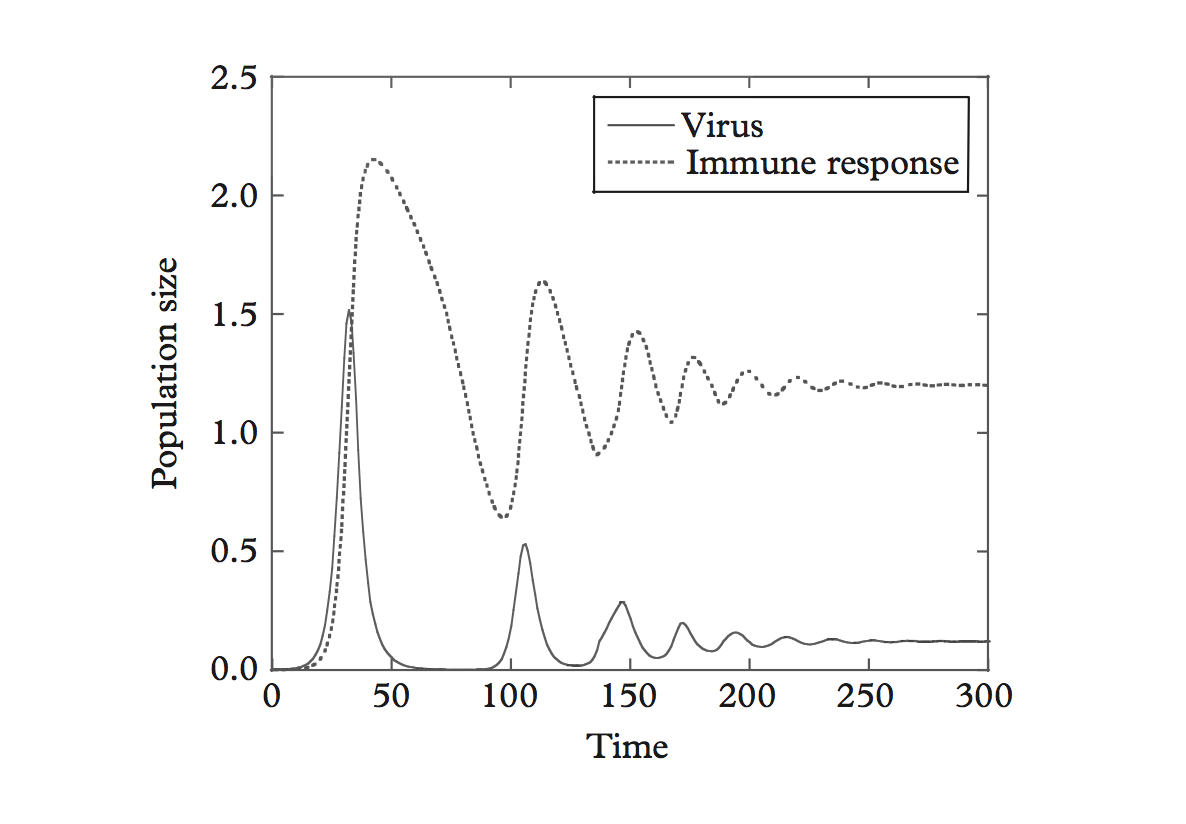
\includegraphics[scale=.4]{imgs/hiv_graph1.png}
    \end{figure}
\end{document}
